\classheader{2018-09-12}
\begin{itemize}
	\item Binary data- special case.
	\item Approximate distance of $\bX$ when $n$ is large but $n << N$
	\item Estimating population Variance
	\item Bivariate data
\end{itemize}
Recall that population is \underline{dichotomous} or \underline{binary} then $x_i = \begin{cases}
	1\\0
\end{cases}$\\
Moreover if we consider $x_i = 1$ as a "success" and $x_i = 0$ as a "failure", then
\begin{equation*}
	\mu = \frac{\sum_{i=1}^N X_i}{N} = \frac{\text{\# of successess in population}}{\text{population size}} = p \tag{$\text{pop}^n$ proportion of success}
\end{equation*}
\begin{gather*}
	\text{Now,} \quad \sigma^2 = \underbrace{\frac{\sum_{i=1}^N X_i}{N}}_{\mu} - \mu^2 = p - p^2 = p(1-p) = pq\\ \begin{align*}
				\mu \text{ as } & 1 \Rightarrow 1^2 = 1
				& 0 \Rightarrow 0^2 = 0
	\end{align*}
\end{gather*}
Recall that if $Y \sim \text{Bernoulli}(p)$, $Y_i = \begin{cases}
	1 & \text{w/ prob } p\\0 & \text{w/ prob } 1-p
\end{cases}$\\
\begin{gather*}
	E[Y] = p\\
	Var(Y) = p(1-p)
\end{gather*}
Last few weeks involved an analysis of $\bX$, $E(\bX)$, $Var(\bX)$. Could also ask: How is $\bX$ distributed if $n$ is large.
\subsection*{Confidence Intervals - Sampling W.R.}
If sampling \textbf{with replacement}, where $X_1, \ldots, X_n$ denotes sample, we know $X_i$'s are $i.i.d.$ Hence when $n$ is large, by CLT $\bX$ has an approximately normal distribution.
\begin{equation*}
	P \bigg(\frac{\bX - \mu}{\sigma/ \sqrt{n}} \leq x \bigg) \longrightarrow \Phi(x) \qquad \text{as } n \rightarrow \infty
\end{equation*}
When sampling with replacement, we can use this to obtain confidence intervals for $\mu$: Let $\alpha \in (0,1)$ be given.
\begin{center}
	Let $Z_\alpha \in \mathbb{R}$ such that $P(Z > Z_\alpha) = \alpha$ where $Z \sim N(0,1)$
\end{center}
By the Central Limit Theorem, for $n$ large (sampling w/replacement)
\begin{gather*}
	= P \bigg( - Z_{\alpha / 2} \leq \frac{\bX - \mu}{\sigma/ \sqrt{n}} \leq Z_{\alpha / 2} \bigg)\\
	= P \bigg(\underbrace{\bX - Z_{\alpha / 2}\cdot \frac{\sigma}{\sqrt{n}}}_{\text{Random}} \leq \mu \leq \underbrace{\bX + Z_{\alpha / 2}\cdot \frac{\sigma}{\sqrt{n}}}_{\text{Random}} \bigg)\\
	Var(\bX) = 0 \qquad \text{Never happens}
\end{gather*}
\begin{center}
	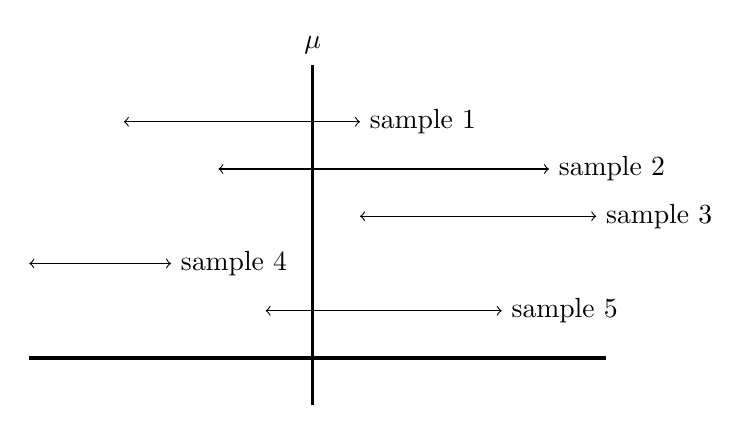
\begin{tikzpicture}[scale=0.6]
    		\draw[very thick,-] (-6,0) -- (6.2,0);
		    \draw[very thick,-] (0,-1) -- (0,6.2) node[above] {$\mu$};

			\draw[<->] (-4,5) -- (1,5) node[right] {sample 1};			
			\draw[<->] (-2,4) -- (5,4) node[right] {sample 2};
			\draw[<->] (1,3) -- (6,3) node[right] {sample 3};
		    \draw[<->] (-6,2) -- (-3,2) node[right] {sample 4};
		    \draw[<->] (-1,1) -- (4,1) node[right] {sample 5};
			\end{tikzpicture}
\end{center}
In repeated sampling, approx $(1 - \alpha)$ of intervals contain $\mu$, and ($\alpha$) frac will not.
\begin{center}
	We say $\boxed{\bX - Z_{\alpha / 2}\cdot \frac{\sigma}{\sqrt{n}}}$ is $100(1-\alpha)$\% 2-sided confidence interval for $\mu$
\end{center}
\textbf{Problem: }This interval involved $\sigma$ which is unknown. Observe that if $n$ is large, then $\frac{\bX - \mu}{\sigma/ \sqrt{n}}$ is still approx $N(0,1)$ in distribution where (no population parameters)
\begin{gather*}
	\tcbhighmath[drop fuzzy shadow]{s^2 = \frac{1}{n-1} \sum(X_i - \bX)^2} \tag{sample variance}
\end{gather*}
So we obtain 
\begin{gather*}
	\tcbhighmath[drop fuzzy shadow]{\bX \pm Z_{\frac{\alpha}{2}} \frac{s}{\sqrt{n}}} \qquad \text{as a $100(1-\alpha)$ CI for $\mu$}
\end{gather*}
\redhline\\\\
In the dichotomous case, 
\begin{gather*}
	\bX = \frac{\text{\# of the succession sample}}{\text{sample size}} = \hat{p}\\
	100(1-\alpha)\% \text{ CI for } \qquad p: \hat{p} \pm Z_{\frac{\alpha}{2}} \sqrt{\frac{\hat{p}(1-\hat{p})}{n}}
\end{gather*}
\subsection*{Confidence Intervals - Sampling W.o.R.}
Recall now what happens when sampling \textbf{without replacement}
\begin{center}
	Here, $X_1, X_2, \ldots, X_n$ remain identically distributed, but not independent
\end{center}
We surmised, that if $n << N$, $X_i \& X_j$ have an \textit{"approximate independence"}
\begin{example-N}
	Let population consist of 1000 elements. In this case:
	\begin{gather*}
		\text{blue } - \circled{1} - 200, \qquad \text{red } - \circled{2} - 300, \qquad \text{green } - \circled{1} - 500\\
		\begin{rcases}
		P(X_1 = \circled{3}) = \frac{1}{2}\\
		P(X_2 = \circled{3} | X_1 = \circled{3}) = \frac{499}{999}
		\end{rcases} \text{not independent, but have approximate independence.}
	\end{gather*}
\end{example-N}
In short, $n << N$, each successive draw does not alter probabilities that much, precisely b/c removal is only of a sample \# of population elements.\\
So if $n << N$, then even in sampling W.O.R, $X_i$'s retain an approximate independence. Further if $n$ is "large" and small relative to $N$, (note delicate point!) then $\bX$ will still have an approx Normal distribution.
\begin{gather*}
	\mathlarger{\frac{\bX - \mu}{\sqrt{\frac{\sigma^2}{n} \big(\frac{N-n}{N-1} \big)}}} \sim N(0,1)
\end{gather*}
Observe $\sigma^2$ us still unknown. We'd like to consider estimators for $\sigma^2$
\subsection*{Estimator for variance W.o.R}
\begin{gather*}
	\hat{\sigma}^2 = \frac{1}{n} \sum_{i = 1}^n (X_i - \bX)^2\\
	s^2 = \frac{1}{n-1} \sum_{i = 1}^n (X_i - \bX)^2
\end{gather*}
Try to understand $E[\hat{\sigma}^2]$
\begin{gather*}
	\hat{\sigma}^2 = \frac{1}{n} \sum_{i = 1}^n (X_1^2 -2X_i \bX + \bX^2)\\
	\hat{\sigma}^2 = \frac{1}{n}\sum\limits_{i=1}^n x_i^2 - 2\bX \bX	 + \bX^2 = \frac{1}{n}\sum\limits_{i=1}^n X_i^2 - \bX^2\\
	E[\hat{\sigma}^2] = \underbrace{E \bigg[\frac{1}{n} \sum\limits_{i=1}^n X_i^2 \bigg]}_{\circled{1}} - \underbrace{E[\bX^2]}_{\circled{2}} \qquad \text{can get $E[\bX^2]$ from $Var(\bX)$}\\
	\begin{split}
		\circled{1} \quad E \bigg[\frac{1}{n} \sum_{i=1}^n X_i^2 \bigg] = \frac{1}{n} \sum_{i=1}^n E[X_i^2] = \sigma^2 + \mu^2\\ 
		%TODO: Why?
	\end{split} \hspace{4em} 
	\begin{split}
	\circled{2} \quad Var(\bX) = E[\bX^2] - (E[\bX])^2\\
		E[\bX^2] = \underbrace{Var(\bX)}_{\text{computed}} + \mu^2\\
	\end{split}\\
	\text{Combining, we get: }\\
	E[\hat{\sigma}^2] = \sigma^2 + \mu^2 - (Var(\bX) + \mu^2)\\
	E[\hat{\sigma}^2] = \sigma^2 - \bigg[\frac{\sigma^2}{n} \bigg(\frac{N-n}{N-1} \bigg) \bigg]
\end{gather*}
The estimator is biased, but
\begin{gather*}
	E[\hat{\sigma}^2] = \sigma^2 \bigg(\underbrace{1 - \frac{N-n}{(n)(N-1)}}_{\text{constant, }c} \bigg)\\
	E[\hat{\sigma}^2] = C \sigma^2
\end{gather*}
and thus $\frac{\hat{\sigma}^2}{C}$ is an unbiased estimator.
